\documentclass{article}
\usepackage[margin=1in]{geometry}
\usepackage{amsmath,amsthm,amssymb}
\usepackage{bbm,enumerate,mathtools}
\usepackage{tikz,pgfplots}
\usepackage{chessboard}
\usepackage[hidelinks]{hyperref}
\usepackage{multicol} % Problem 35

\newenvironment{question}{\begin{trivlist}\item[\textbf{Question.}]}{\end{trivlist}}
\newenvironment{note}{\begin{trivlist}\item[\textbf{Note.}]}{\end{trivlist}}
\newenvironment{references}{\begin{trivlist}\item[\textbf{References.}]}{\end{trivlist}}
\newenvironment{related}{\begin{trivlist}\item[\textbf{Related.}]\end{trivlist}\begin{enumerate}}{\end{enumerate}}


\begin{document}
\rating{3}{4}
Let a ``popsicle stick weave'' be a configuration of lines segments, called ``sticks'', such that
\begin{enumerate}[(1)]
  \item when you lift up any stick by the end, the structure supports itself (is in tension)
  \item the removal of any stick results in a configuration that no longer supports itself.
\end{enumerate}

\begin{figure}[!h]
  \centering
  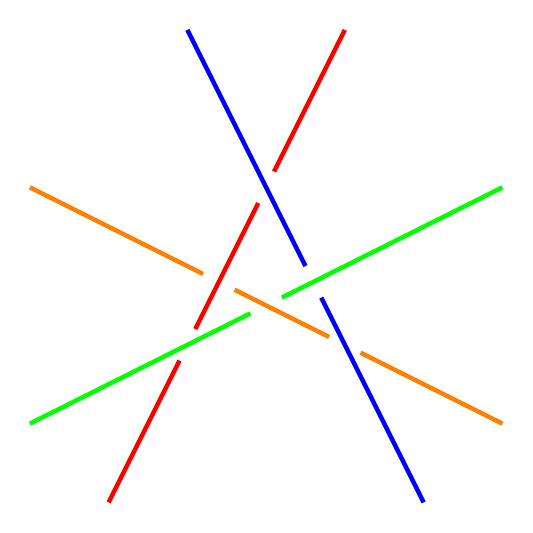
\begin{tikzpicture}
    % red(x) = 2x - 2
    \draw[ultra thick, red] (1,0) -- (1.9, 1.8);
    \draw[ultra thick, red] (2.1, 2.2) -- (2.9,3.8);
    \draw[ultra thick, red] (3.1,4.2) -- (4,6);
    % blue(x) = -2x + 10
    \draw[ultra thick, blue] (5,0) -- (3.7,2.6);
    \draw[ultra thick, blue] (3.5,3) -- (2,6);
    % green(x) = (1/2)x + 1
    \draw[ultra thick, green] (0,1) -- (2.8,2.4);
    \draw[ultra thick, green] (3.2,2.6) -- (6,4);
    % orange(x) = (-1/2)x + 4
    \draw[ultra thick, orange] (0,4) -- (2.2,2.9);
    \draw[ultra thick, orange] (2.6,2.7) -- (3.8,2.1);
    \draw[ultra thick, orange] (4.2,1.9) -- (6,1);
  \end{tikzpicture}
  \caption{The unique example of a 4 stick crossing (up to reflection)}
\end{figure}

\begin{figure}[!h]
  \centering
  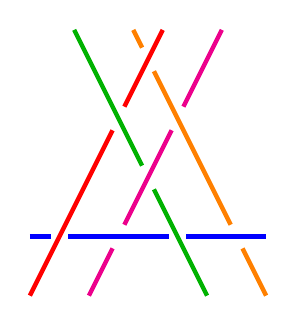
\begin{tikzpicture}[scale=0.375]
    \draw[ultra thick, draw=red, domain=0:2.8] plot ({\x}, {2*\x});
    \draw[ultra thick, draw=red, domain=3.2:4.5] plot ({\x}, {2*\x});

    \draw[ultra thick, draw=magenta, domain=2:2.8] plot ({\x}, {2*\x - 4});
    \draw[ultra thick, draw=magenta, domain=3.2:4.8] plot ({\x}, {2*\x - 4});
    \draw[ultra thick, draw=magenta, domain=5.2:6.5] plot ({\x}, {2*\x - 4});

    \draw[ultra thick, draw=black!30!green, domain=1.5:3.8] plot ({\x}, {-2*\x + 12});
    \draw[ultra thick, draw=black!30!green, domain=4.2:6] plot ({\x}, {-2*\x + 12});

    \draw[ultra thick, draw=orange, domain=3.5:3.8] plot ({\x}, {-2*\x + 16});
    \draw[ultra thick, draw=orange, domain=4.2:6.8] plot ({\x}, {-2*\x + 16});
    \draw[ultra thick, draw=orange, domain=7.2:8] plot ({\x}, {-2*\x + 16});

    \draw[ultra thick, draw=blue, domain=0:0.7] plot ({\x}, {2});
    \draw[ultra thick, draw=blue, domain=1.3:4.7] plot ({\x}, {2});
    \draw[ultra thick, draw=blue, domain=5.3:8] plot ({\x}, {2});
  \end{tikzpicture}
  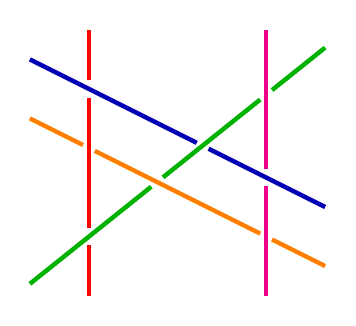
\begin{tikzpicture}[scale=0.375]
    \draw[ultra thick, draw=red, domain=0:1.7] plot ({2}, {\x});
    \draw[ultra thick, draw=red, domain=2.3:6.7] plot ({2}, {\x});
    \draw[ultra thick, draw=red, domain=7.3:9] plot ({2}, {\x});

    \draw[ultra thick, draw=magenta, domain=0:3.7] plot ({8}, {\x});
    \draw[ultra thick, draw=magenta, domain=4.3:9] plot ({8}, {\x});

    \draw[ultra thick, draw=black!30!green, domain=0:4.11] plot ({\x}, {0.8*\x + 0.4});
    \draw[ultra thick, draw=black!30!green, domain=4.51:7.8] plot ({\x}, {0.8*\x + 0.4});
    \draw[ultra thick, draw=black!30!green, domain=8.2:10] plot ({\x}, {0.8*\x + 0.4});

    \draw[ultra thick, draw=orange, domain=0:1.8] plot ({\x}, {-0.5*\x + 6});
    \draw[ultra thick, draw=orange, domain=2.2:7.8] plot ({\x}, {-0.5*\x + 6});
    \draw[ultra thick, draw=orange, domain=8.2:10] plot ({\x}, {-0.5*\x + 6});

    \draw[ultra thick, draw=black!30!blue, domain=0:5.65] plot ({\x}, {-0.5*\x + 8});
    \draw[ultra thick, draw=black!30!blue, domain=6.05:10] plot ({\x}, {-0.5*\x + 8});
  \end{tikzpicture}
  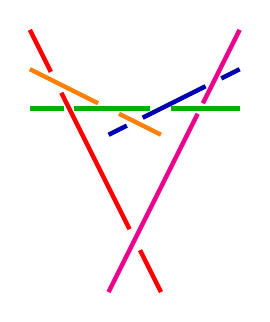
\begin{tikzpicture}[scale=0.333]
    \draw[ultra thick, draw=red, domain=0:0.8] plot ({\x}, {-2*\x + 10});
    \draw[ultra thick, draw=red, domain=1.2:3.8] plot ({\x}, {-2*\x + 10});
    \draw[ultra thick, draw=red, domain=4.2:5] plot ({\x}, {-2*\x + 10});

    \draw[ultra thick, draw=magenta, domain=3:6.4] plot ({\x}, {2*\x - 6});
    \draw[ultra thick, draw=magenta, domain=6.6:8] plot ({\x}, {2*\x - 6});

    \draw[ultra thick, draw=black!30!green, domain=0:1.3] plot ({\x}, {7});
    \draw[ultra thick, draw=black!30!green, domain=1.7:4.6] plot ({\x}, {7});
    \draw[ultra thick, draw=black!30!green, domain=5.4:8] plot ({\x}, {7});

    \draw[ultra thick, draw=orange, domain=0:2.6] plot ({\x}, {-0.5*\x + 8.5});
    \draw[ultra thick, draw=orange, domain=3.4:5] plot ({\x}, {-0.5*\x + 8.5});

    \draw[ultra thick, draw=black!30!blue, domain=3:3.7] plot ({\x}, {0.5*\x + 4.5});
    \draw[ultra thick, draw=black!30!blue, domain=4.3:6.7] plot ({\x}, {0.5*\x + 4.5});
    \draw[ultra thick, draw=black!30!blue, domain=7.3:8] plot ({\x}, {0.5*\x + 4.5});
  \end{tikzpicture}
  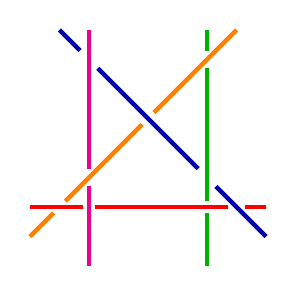
\begin{tikzpicture}[scale=0.375]
    \draw[ultra thick, draw=red, domain=0:1.8] plot ({\x}, {2});
    \draw[ultra thick, draw=red, domain=2.2:6.7] plot ({\x}, {2});
    \draw[ultra thick, draw=red, domain=7.3:8] plot ({\x}, {2});

    \draw[ultra thick, draw=magenta, domain=0:2.7] plot ({2}, {\x});
    \draw[ultra thick, draw=magenta, domain=3.3:8] plot ({2}, {\x});

    \draw[ultra thick, draw=black!30!green, domain=0:1.8] plot ({6}, {\x});
    \draw[ultra thick, draw=black!30!green, domain=2.2:6.7] plot ({6}, {\x});
    \draw[ultra thick, draw=black!30!green, domain=7.3:8] plot ({6}, {\x});

    \draw[ultra thick, draw=orange, domain=0:0.8] plot ({\x}, {\x + 1});
    \draw[ultra thick, draw=orange, domain=1.2:3.8] plot ({\x}, {\x + 1});
    \draw[ultra thick, draw=orange, domain=4.2:7] plot ({\x}, {\x + 1});

    \draw[ultra thick, draw=black!30!blue, domain=1:1.7] plot ({\x}, {-\x + 9});
    \draw[ultra thick, draw=black!30!blue, domain=2.3:5.7] plot ({\x}, {-\x + 9});
    \draw[ultra thick, draw=black!30!blue, domain=6.3:8] plot ({\x}, {-\x + 9});

  \end{tikzpicture}
  \caption{
    Four of five (?) known examples of five-stick crossings.
    Perhaps the fourth example shouldn't count, because shortening the blue
    stick to avoid the blue-red crossing results in a valid configuration
    (the remaining known five-stick crossing).
  }
\end{figure}

\begin{question}
  How many distinct popsicle stick weaves exist for $n$ sticks?
\end{question}

\begin{related}
  \item What if the sticks are only allowed to touch three other sticks?
  \item What if the sticks are another geometric object (e.g. semicircles)?
\end{related}
\end{document}
